\section{Motivação}
\label{motivacao}

O estudo de linguagens menores que sejam capazes de expressar regras de maneira mais clara não é novidade na área da engenharia de sistemas, \citeonline{bentley} já demonstrava em seu estudo diferentes abordagens de construção de pequenas linguagens para facilitar a escrita de programas gráficos e interface gráfica. \citeonline{wexelblat} apresenta o termo "linguagem de propósito especial", quando se refere à \gls{JOVIAL}, linguagem de alto nível destinada principalmente para auxiliar na programação de grandes sistemas complexos em tempo real. 

Um exemplo de aplicação dessas linguagens pode ser visto na Figura \ref{fig:piclanguage} onde o compilador transforma comandos simples no formato textual em formato de digrama (Figura \ref{fig:piclanguageresultado}), abstraindo detalhes específicos das linguagens tradicionais de programação da época.

\begin{figure}[ht!]
\centering

\caption{\textmd{Comandos na PIC Language}}
\label{fig:piclanguage}
\fcolorbox{gray}{white}{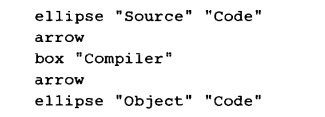
\includegraphics[width=0.67\textwidth]{images/piclanguage}}

\par\medskip\textbf{Fonte:} \citeonline{bentley}. \par\medskip
\end{figure}

\begin{figure}[ht!]
\centering

\caption{\textmd{Diagrama resultado após compilação}}
\label{fig:piclanguageresultado}
\fcolorbox{gray}{white}{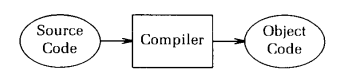
\includegraphics[width=0.67\textwidth]{images/piclanguageresultado}}

\par\medskip\textbf{Fonte:} \citeonline{bentley}. \par\medskip
\end{figure}



Na engenharia de software atual, as Linguagens de Domínio Específico ou DSL estão se tornando cada vez mais importantes e as novas ferramentas de criação dessas linguagens são ainda melhores, pois requerem esforço de desenvolvimento relativamente simples \cite{dslengineering}.


Hoje a equipe de desenvolvedores do \gls{IFSC} possui uma alta demanda de desenvolvimento de sistemas e serviços internos, atualmente são mantidos mais de 10 sistemas em uso, alguns deles são subdivididos em vários módulos \cite{catalogoifsc}. A equipe da \gls{DTIC} que mantém os sistemas, conta com apenas 12 analistas da tecnologia da informação, além de ter que prestar suporte para todas as 23 unidades da instituição, pois a gestão centraliza todos os serviços de TI nesse departamento. 

Como agravante o sistema de ingresso, foco deste trabalho, foi criado em meados dos anos 2000 por bolsistas que já não estão mais na instituição, e apenas 2 desenvolvedores ficaram responsáveis pelas demandas de desenvolvimento e suporte. Por se tratar de um sistema legado criado em linguagem PHP sem qualquer preocupação com documentação ou qualidade de código, o custo de alterações mais complexas como no caso de regras de classificação acaba por atrasar a adequação aos novos requisitos de lei. 

Até o momento a equipe participou do desenvolvimento de 3 versões do algoritmo de classificação, além de prestar manutenção corretiva em função de entendimentos equivocados nas regras implementadas.  Os algoritmos envolvidos, assim como o seu histórico de versionamento serão detalhados na subseção \ref{historicoversoes}.

Nesse contexto, o presente trabalho apresenta como proposta uma Linguagem de Domínio Específico para especificação de regras de classificação de candidatos, de modo mais alto nível, onde usuários especialistas do sistema de ingresso possam estabelecer as categorias de cotas, com objetivo de reduzir o esforço do desenvolvimento e de entendimento das regras de negócio, por parte dos desenvolvedores do sistema, sempre que forem alterados os documentos de lei envolvidos.

\chapter{Sistema de Ingresso e Versionamento}
\label{historicoversoes}

Neste capítulo serão descritas informações sobre as funcionalidades desenvolvidas no sistema de ingresso do \gls{IFSC} com relação aos requisitos e algoritmos do sistema de cotas, para este fim será utilizado o histórico do controle de versão no que concerne ao quantitativo de arquivos, classes, funções/métodos e as diferentes versões desde o surgimento da demanda de cotas na legislação.

\section{Histórico de Projeto}
\label{historicopj}
Criado em meados do ano de 2000 o sistema tem por objetivo disponibilizar vagas de cursos para os discentes do \gls{IFSC}. Este sistema foi desenvolvido internamente na linguagem PHP, para automatizar os processos seletivos, que eram realizados por meio de planilhas e ferramentas não integradas, as quais demandavam ao setor responsável muitas pessoas e muitos procedimentos operacionais repetitivos, gerando falhas no processo por erro humano.

O projeto não utiliza conceitos de orientação a objetos, em sua maioria os arquivos PHP ultrapassam duas mil linhas, sem divisão em camadas \gls{MVC}, com combinações das linguagens Javascript, HTML e PHP no mesmo arquivo. Quando era preciso criar ou adaptar alguma nova funcionalidade, por falta de conhecimento técnico os antigos desenvolvedores (bolsistas) faziam a cópia das funcionalidades para vários locais do sistema, sem pensar em reutilização de código.

Com objetivo de elencar a situação atual do código fonte do sistema, neste trabalho serão apresentados os quantitativos levantados a partir do sistema de controle de versão do \gls{IFSC}. O Quadro \ref{quadro_git_ingresso} apresenta o levantamento geral sobre o total de arquivos, linhas de código, commits e desenvolvedores que já atuaram no projeto. Nas seções seguintes serão contextualizados os dados gerais sobre o algoritmo de classificação, assim como será descrito o levantamento feito nas 3 (três) versões do algoritmo de classificação que foram implementadas até o momento.

\begin{quadro}
\caption{Dados gerais do controle de versão}
\label{quadro_git_ingresso}
\centering
\begin{tabular}{ l l }
   \cline{1-1}\cline{2-2}  
    \multicolumn{1}{|p{5.850cm}|}{\textbf{Total de arquivos}} &
    \multicolumn{1}{p{8.217cm}|}{1.357 arquivos (php, html, css, js )}
  \\ 
   \cline{1-1}\cline{2-2}  
    \multicolumn{1}{|p{5.850cm}|}{\textbf{Total de linhas de código}} &
    \multicolumn{1}{p{8.217cm}|}{36.9414 linhas}
  \\    
   \cline{1-1}\cline{2-2}  
    \multicolumn{1}{|p{5.850cm}|}{\textbf{Total de commits}} &
    \multicolumn{1}{p{8.217cm}|}{731}
  \\    
   \cline{1-1}\cline{2-2}  
    \multicolumn{1}{|p{5.850cm}|}{\textbf{Total de desenvolvedores}} &
    \multicolumn{1}{p{8.217cm}|}{6}
  \\     
   \cline{1-1}\cline{2-2}  
    \multicolumn{1}{|p{5.850cm}|}{\textbf{Período da coleta}} &
    \multicolumn{1}{p{8.217cm}|}{11/02/2015 - 17/04/2019}
  \\       
  \hline

 \end{tabular} 
\end{quadro}

\section{Algoritmo de Classificação}
\label{algoritimodeclassificacao}

Neste seção serão detalhados os conceitos e as etapas do processo de classificação de candidatos à vagas do sistema de cotas, assim como o levantamento de cenários exemplifica-tórios sobre distribuição de vagas tendo como base as versões já implementadas no sistema de ingresso.

Para cada processo seletivo há uma lista de cursos, onde o setor que gerencia as vagas define o valor total de vagas iniciais e indica se o processo seletivo vai utilizar a regra de classificação por cotas. Durante as inscrições serão apresentados aos candidatos os campos necessários para indicar que vieram de escola pública e também informar sua renda familiar e se autodeclaram pretos, pardos e indígenas.

Após o término do período de inscrições os candidatos são separados em categorias de concorrência de acordo com o preenchimento realizado no ato da inscrição. A seguir, os candidatos participam do processo seletivo de forma física ( provas de vestibular ) ou eletrônica ( sorteio, pontuação por preenchimento de formulários sócio-econômicos ou classificação por ENEM/SISU ). Por fim é gerado um número de classificação que representa a ordem dos candidatos que disputam as vagas disponíveis.

O algoritmo de classificação utiliza como parâmetro de entrada a lista de candidatos, contendo o número de inscrição, a ordem de classificação geral, a data de nascimento (como critério de desempate), a quantidade de vagas total do curso, o percentual de vagas disponível para escola pública e o percentual de proporção do \gls{IBGE}, que varia conforme a Unidade Federada e é fornecido conforme o ultimo censo demográfico, representando o percentual sobre o total de pretos, pardos e indígenas no estado em relação às demais categorias.

Com esses parâmetros de entrada o algoritmo gera um quadro de vagas contendo quantas vagas estão reservadas para às respectivas categorias de cotas, e faz a seleção e aprovação de candidatos de acordo com a sua classificação e critérios de desempate. Por fim, em caso de sobra de vagas por falta de candidatos para uma determinada categoria de cota, o algoritmo utiliza faz nova busca por candidatos de outra categoria conforme ordem de prioridade estabelecida na portaria Nº 18 de 2012 do \gls{MEC}, a qual define:

\begin{citacao}
Art. 15. No caso de não preenchimento das vagas reservadas aos autodeclarados pretos, pardos
e indígenas e às pessoas com deficiência, aquelas remanescentes serão preenchidas pelos
estudantes que tenham cursado integralmente o ensino fundamental ou médio, conforme o caso,
em escolas públicas, observadas as reservas realizadas em mesmo nível ou no imediatamente
anterior, nos termos do art. 10 desta Portaria. \cite{portarianr9}
\end{citacao}

Ao final do processo de classificação é gerada uma lista de candidatos aprovados, incluindo a classificação geral e a classificação na respectiva categoria de cota, por fim esta lista é enviada ao sistema acadêmico para que os candidatos possam realizar a matrícula e entregar a documentação necessária. 

As alterações nos documentos de lei podem incluir novas categorias, novas formas de distribuição das vagas iniciais, mudanças de percentuais, formas de arredondamento, descrição dos tipos de cotas e mudança na ordem de prioridade em caso de sobra de vaga. Deste modo, nas seções seguintes serão relatados os casos e cenários onde no \gls{IFSC} houve maior impacto de refatoração de código para adequação à legislação.


\subsection{Versão 1 - Início do sistema de Cotas, Lei Nº 12.711 de 2012}
\label{versao1}

\subsection{Versão 2 - Alteração para Lei Nº 13.409 de 2016 }
\label{versao1}

\subsection{Versão 3 - Reimplementação para interpretação do MEC em 2017 }
\label{versao1}

\subsection{Outras customizações realizadas no algoritmo}
\label{versao1}